% Created 2021-09-12 Sun 22:49
% Intended LaTeX compiler: xelatex
\documentclass[letterpaper]{article}
\usepackage{graphicx}
\usepackage{grffile}
\usepackage{longtable}
\usepackage{wrapfig}
\usepackage{rotating}
\usepackage[normalem]{ulem}
\usepackage{amsmath}
\usepackage{textcomp}
\usepackage{amssymb}
\usepackage{capt-of}
\usepackage{hyperref}
\usepackage[margin=1in]{geometry}
\usepackage{fontspec}
\usepackage{indentfirst}
\setmainfont[ItalicFont = LiberationSans-Italic, BoldFont = LiberationSans-Bold, BoldItalicFont = LiberationSans-BoldItalic]{LiberationSans}
\newfontfamily\NHLight[ItalicFont = LiberationSansNarrow-Italic, BoldFont       = LiberationSansNarrow-Bold, BoldItalicFont = LiberationSansNarrow-BoldItalic]{LiberationSansNarrow}
\newcommand\textrmlf[1]{{\NHLight#1}}
\newcommand\textitlf[1]{{\NHLight\itshape#1}}
\let\textbflf\textrm
\newcommand\textulf[1]{{\NHLight\bfseries#1}}
\newcommand\textuitlf[1]{{\NHLight\bfseries\itshape#1}}
\usepackage{fancyhdr}
\pagestyle{fancy}
\usepackage{titlesec}
\usepackage{titling}
\makeatletter
\lhead{\textbf{\@title}}
\makeatother
\rhead{\textrmlf{Compiled} \today}
\lfoot{\theauthor\ \textbullet \ \textbf{2021-2022}}
\cfoot{}
\rfoot{\textrmlf{Page} \thepage}
\titleformat{\section} {\Large} {\textrmlf{\thesection} {|}} {0.3em} {\textbf}
\titleformat{\subsection} {\large} {\textrmlf{\thesubsection} {|}} {0.2em} {\textbf}
\titleformat{\subsubsection} {\large} {\textrmlf{\thesubsubsection} {|}} {0.1em} {\textbf}
\setlength{\parskip}{0.45em}
\renewcommand\maketitle{}
\author{Houjun Liu}
\date{\today}
\title{Virus Infections and Lifecycle}
\hypersetup{
 pdfauthor={Houjun Liu},
 pdftitle={Virus Infections and Lifecycle},
 pdfkeywords={},
 pdfsubject={},
 pdfcreator={Emacs 28.0.50 (Org mode 9.4.4)}, 
 pdflang={English}}
\begin{document}

\maketitle


\section{Virus Infections and Lifecycle}
\label{sec:org98d69c9}
\subsection{Viral Life Cycle, an Overview}
\label{sec:orgd318d88}
\begin{enumerate}
\item \textbf{Attachment} => protein contact between virus and host
\item \textbf{Viral entry} => entering the cell
\item \textbf{Uncoating} => shedding the protein layer
\item \textbf{Biosynthesis} => make baby viruses

\begin{enumerate}
\item Genome Replication: transcribe DNA/RNA
\item Genome Expression: read DNA/RNA to make proteins
\end{enumerate}

\item \textbf{Genome integration} => retrovirus only --- put the viral gene into
the genetic sequence of the actual cell
\item \textbf{Assembly} => put it all together
\item \textbf{Viral Exit} => mature virons leave
\end{enumerate}

\subsection{Viral attachment}
\label{sec:org98cb17f}
To be able to enter a cell, viruses have to do something to stick to it.
B/c otherwise they would just be stuck in the bloodstream and be very
sad.

See \href{KBhBIO101ViralAttachment.org}{KBhBIO101ViralAttachment}

\subsection{Viral Entry}
\label{sec:orgdcf6e99}
In this step, the sticky virus on the surface of the cell gets into the
cell. There are three different types of mechanisms by which this is
achieved.

See \href{KBhBIO101ViralEntry.org}{KBhBIO101ViralEntry}

\subsection{Uncoating}
\label{sec:org19c8c27}
After the virus enters the cell, the lipid/protein shell on the outside
must be shred to be able to release the additional DNA inside.

See \href{KBhBIO101ViralUncoating.org}{KBhBIO101ViralUncoating}

\subsection{Viral Replication}
\label{sec:org332a4ba}
Now, with the viruses's DNA out on full display inside the cell, how do
we make another virus? There are two key questions that must be asked to
answer this:

\begin{itemize}
\item \textbf{How are viral mRNAs produced from the viral genome?} => virus will
hijack the ribosomes in the host cells. So, it is more important to
ask how the mRNAs are produced to tell ribosomes what to do
\item \textbf{What serves as the template for viral genome replication} =>
replication will need a polymeraese; but the source and mechanism is
dependent on viral genome structure/composition
\end{itemize}

\begin{figure}[htbp]
\centering
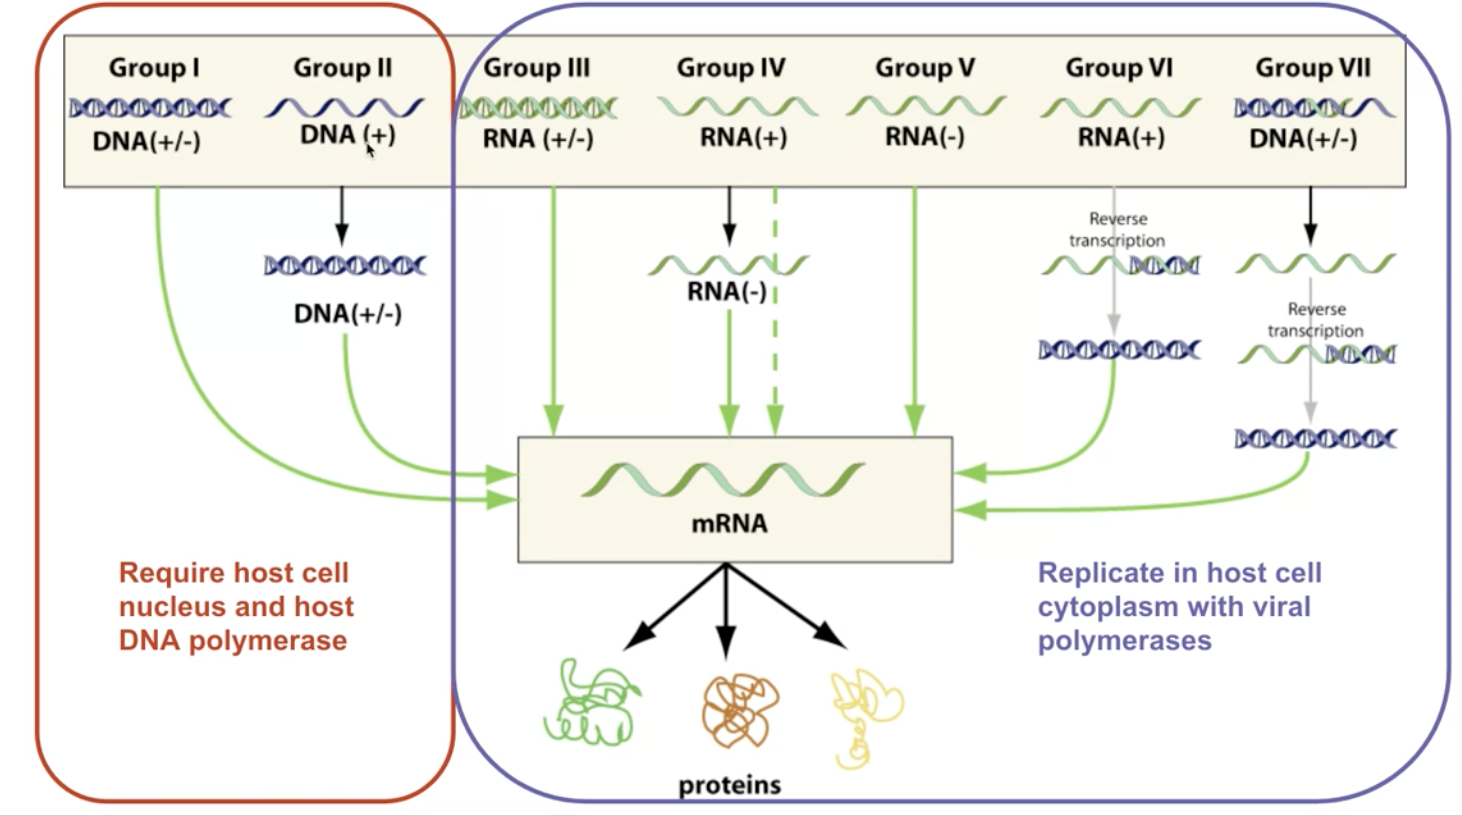
\includegraphics[width=.9\linewidth]{Screen Shot 2020-10-12 at 11.04.53 PM.png}
\caption{Screen Shot 2020-10-12 at 11.04.53 PM.png}
\end{figure}

See \href{KBhBIO101ViralReplication.org}{KBhBIO101ViralReplication}

\subsection{Packaging}
\label{sec:org77eeba9}
"Viral self-assembly" --- make the protein, and, without ATP, just seal
the newly-formed virus DNA in.

\subsection{Viral Exit}
\label{sec:org4bc8a3b}
This is the process by which mature viron exit the host cell. See
\href{KBhBIO101ViralExit.org}{KBhBIO101ViralExit}
\end{document}
